\documentclass[conference]{IEEEtran}
\IEEEoverridecommandlockouts

\usepackage{cite}
\usepackage{amsmath,amssymb,amsfonts}
\usepackage{graphicx}
\usepackage{url}
\usepackage{textcomp}
\usepackage{xcolor}
\usepackage{booktabs}
\usepackage{array}
\usepackage{tabularx}

\def\BibTeX{{\rm B\kern-.05em{\sc i\kern-.025em b}\kern-.08em
    T\kern-.1667em\lower.7ex\hbox{E}\kern-.125emX}}

\begin{document}

\title{Analysis of the Islamic Scholarly Network in the Hadith
\textit{Sanad} Using Knowledge Graph and Social Network Analysis
with an Interactive Dashboard Visualization}

\author{\IEEEauthorblockN{1\textsuperscript{st} Moh. Nazril Ilham}
\IEEEauthorblockA{\textit{Department of Electrical and}\\
\textit{Information Engineering}\\
\textit{Universitas Gadjah Mada}\\
Yogyakarta, Indonesia\\
mohnazrililham@mail.ugm.ac.id}
\and
\IEEEauthorblockN{2\textsuperscript{nd} Widyawan}
\IEEEauthorblockA{\textit{Department of Electrical and}\\
\textit{Information Engineering}\\
\textit{Universitas Gadjah Mada}\\
Yogyakarta, Indonesia\\
widyawan@ugm.ac.id}
\and
\IEEEauthorblockN{3\textsuperscript{rd} Guntur Dharma Putra}
\IEEEauthorblockA{\textit{Department of Electrical and}\\
\textit{Information Engineering}\\
\textit{Universitas Gadjah Mada}\\
Yogyakarta, Indonesia\\
gdputra@ugm.ac.id}}

\maketitle

\begin{abstract}
The hadith \textit{sanad} is an Islamic scholarly network formed by chains of
teacher--student relationships among narrators across generations, a relational
structure that lends itself naturally to directed-graph modeling. Prior studies
have applied Knowledge Graph (KG) and Social Network Analysis (SNA) methods to
\textit{sanad} networks, but their outputs are static, rendered at full scale in
generic graph terminology, and operable only through desktop software such as
Gephi and Cytoscape, so hadith students and researchers---the very audience that
routinely traces narrator standing---must still work through \textit{rijal}
literature sequentially by hand. This paper analyzes the Islamic scholarly
network of the \textit{sanad} as a KG with SNA and presents the analysis through
a publicly accessible interactive web dashboard. From the Sanadset~650K corpus
(650{,}986 hadith entries from 926 classical Arabic books), 487{,}451 cleaned
\textit{sanad} chains were modeled as a weighted directed graph of 177{,}047
narrator nodes and 776{,}798 narration edges. In-degree, out-degree, and
eigenvector centrality were computed on the full graph; closeness and betweenness
were computed on a 14{,}695-node strongest-weight subgraph. Abu Hurairah ranks
first in four of five metrics while Sufyan leads in out-degree, a role split that
matches classical biographical assessments. The residual risk of identity merging
introduced by kinship-term resolution was quantified rather than assumed, and is
concentrated in 9.85\% of the 102{,}100 resolution events. Building and analyzing
the full graph takes about 13~s for loading, construction, and the degree- and
eigenvector-based metrics, with a 701.4~MB peak RSS. The dashboard, built with
React over a Supabase (PostgreSQL) backend and an HTML5 Canvas force-directed
graph, passed 14 of 14 black-box scenarios, sustained 57--61 FPS during graph
interaction, and scored 71.23 on an adapted seven-item System Usability Scale
with 18 respondents.
\end{abstract}

\begin{IEEEkeywords}
knowledge graph, hadith sanad, social network analysis, narrator centrality,
network visualization, interactive dashboard
\end{IEEEkeywords}

% =============================================================
\section{Introduction}
% =============================================================

Hadith, the recorded sayings, actions, and tacit approvals of the Prophet
Muhammad, is the second source of Islamic law after the Qur'an
\cite{handayani2026hadis,hatta2026teknik}. Structurally, a hadith consists of two
components: the \textit{matn} (the text itself) and the \textit{sanad}, the
continuous chain of narrators who transmitted the text across generations. The
\textit{sanad} forms an Islamic scholarly network built from teacher--student
relationships, in which each narrator is a link in the intergenerational transfer
of religious knowledge \cite{Mustang_Abubakar_2025}. A narrator is conventionally
identified by tracing the list of their teachers and students together with their
generation (\textit{tabaqat}) \cite{WanKamalNadzif2025135}, so a \textit{sanad} is
naturally represented as a directed graph with narrators as nodes and
teacher--student relations as edges \cite{FAROOQI2024110439}.

Mapping this network accurately is not straightforward. The source material is
classical Arabic text with high orthographic variance in narrator names---presence
or absence of diacritics, alternate Unicode letterforms, contextual kinship terms,
and the \textit{kunyah} forms \textit{Abu}, \textit{Abi}, and \textit{Aba}---so
without careful handling one narrator is recorded as several distinct entities.
That complexity is compounded by scale: hundreds of thousands of transmission
entries drawn from hundreds of books \cite{MGHARI2022108540}, which makes manual
tracing impractical.

Not all narrators play an equal role. Some occupy strategic positions as
convergence points traversed by many \textit{sanad} paths, known as
\textit{common links} \cite{mufid2023track}. Classical scholarship identifies them
manually through \textit{isnad}-bundle analysis, but at the scale of hundreds of
thousands of narrators this is inadequate. Simple text search is no shortcut
either: it returns a single occurrence count without capturing a narrator's
structural position, a limitation consistent with the broader challenge of
large-scale information retrieval, which demands richer data representations than
string matching \cite{rixewa2024interleaved}.

Over the past decade this need has been addressed by quantitative studies of the
narrator network: reconstructing temporal information from transmission structure
\cite{Shuaib2022}, representing the network as a Knowledge Graph (KG)
\cite{FAROOQI2024110439}, and applying centrality metrics together with
exploratory visualization prototypes \cite{Mghari2024Narrator2Vec}. These studies
generally rely on desktop analysis tools such as Gephi and Cytoscape
\cite{FAROOQI2024110439}, and their outputs are static images or whole-graph files
that are dense and hard to trace at the scale of hundreds of thousands of
narrators. They also remain expressed in generic graph vocabulary (node, edge,
centrality score) without translation into roles meaningful within hadith studies,
such as teacher, student, or \textit{common link}. As a result, a hadith
researcher wishing to trace one narrator's relations across generations must
still do so sequentially and manually through \textit{rijal} literature.

The KG representation nonetheless offers a foundation that can be developed into
a more interactive and accessible system. A KG captures entities and their
relations semantically and has been widely adopted across domains such as
education and tourism to extract insight from large-scale data \cite{Aoula2026}.
For hadith studies, it fits the narration network directly, with narrators as
entities and teacher--student relations as edges \cite{FAROOQI2024110439}.
Turning that network into explorable knowledge requires an interactive web
front-end for three reasons: \emph{visualization scalability}, so a network of
hundreds of thousands of narrators is presented as a representative, progressively
traceable subset rather than one dense static image \cite{LópezWerner04072025};
\emph{semantic accessibility}, so centrality values and graph structure are
translated into terms familiar in hadith studies; and \emph{relational
navigation}, so a narrator's teachers and students can be traversed by
click-through interaction instead of sequential manual lookup. Meeting these
requirements is not merely a matter of choosing a front-end framework, since
interactive graph performance depends heavily on the rendering technology---the
choice between ready-made libraries and native browser primitives (SVG, Canvas,
WebGL) determines whether a visualization stays responsive at thousands of nodes
or stalls at hundreds \cite{Zhao2025}.

This paper analyzes the Islamic scholarly network of the hadith \textit{sanad}
using a KG and SNA over the publicly available Sanadset~650K dataset
\cite{MGHARI2022108540}, and presents the results through an interactive
dashboard. The contributions are fourfold: (i) construction of a large-scale
weighted directed KG of the \textit{sanad} network through systematic
preprocessing, together with a quantitative evaluation of the residual identity
ambiguity that rule-based kinship resolution introduces; (ii) quantitative
identification of narrator roles using five SNA centrality metrics, interpreted
against classical biographical scholarship; (iii) an interactive, publicly
deployed dashboard designed around the stated needs of hadith students and
researchers; and (iv) empirical measurement of the computational cost of building
and analyzing the graph and of the dashboard's runtime behavior, figures that
prior \textit{sanad} network studies do not report.

% =============================================================
\section{Related Work}
% =============================================================

Computational research on the hadith \textit{sanad} has progressed from dataset
construction toward graph-based modeling and SNA. Mghari \textit{et al.}\ built
Sanadset~650K, a corpus of 650{,}986 entries from 926 classical Arabic books, in
which each entry separates the full hadith text, \textit{matn}, narrator list,
and \textit{sanad} ordering \cite{MGHARI2022108540}. Its scale and coverage make
it the most representative source for \textit{sanad} transmission research, though
it is provided as raw data without graph visualization or network analysis. The
same group later proposed Narrator2Vec, a Skip-Gram Word2Vec adaptation that
learns vector representations of narrator names and predicts missing narrators in
broken chains \cite{Mghari2024Narrator2Vec}; it does not, however, produce
per-narrator quantitative scores that users can compare.

Farooqi \textit{et al.}\ introduced Multi-IsnadSet, representing the Sahih Muslim
transmission network as a directed graph of 2{,}092 nodes and 77{,}797 edges,
built and analyzed with NetworkX, Neo4j, Gephi, and Cytoscape
\cite{FAROOQI2024110439}. They demonstrated that a \textit{sanad} network can be
modeled as a KG, and explicitly noted that SNA metrics such as degree,
betweenness, and eigenvector centrality \emph{could} be applied to identify
influential narrators---an analysis they left as future work. Shuaib \textit{et
al.}\ applied trophic analysis to a 49{,}309-narrator hadith network and showed
that the network is hierarchical and sequential, recovering temporal information
from structure \cite{Shuaib2022}, yet without centrality metrics or an interactive
interface. Mahmoud \textit{et al.}\ proposed NarratorsKG, the first KG dedicated
to hadith narrators (79{,}256 nodes, 197{,}183 edges), used for narrator
disambiguation with graph-query embeddings and AraBERT \cite{Mahmoud2024}; it is
an internal NLP resource rather than an end-user system. Hendawi \textit{et al.}\
used machine learning to verify \textit{sanad} continuity from narrator
biographical data \cite{10974901}, reinforcing the value of structured narrator
data.

A parallel line of work visualizes narrator chains as graphs. Sara\c{c}o\u{g}lu
converted 2{,}258 \textit{isnad} chains into source--target pairs and visualized
them with Pajek, Gephi, and Isnalyser \cite{saraccougluvisualization}. HadithNet
automated narrator-name identification and chain generation on a web system using
Django, MySQL, and Graphviz, reaching 99.37\% name precision but struggling with
complex branching chains \cite{alias2024hadithnet}. Ahmad \textit{et al.}\ showed
that transforming \textit{isnad} into directed graphs enables centrality,
clustering, and bridge-narrator analysis \cite{ahmad2025hadith}, and the KASHAF
system offered interactive Sankey-flow visualization over 60{,}000 hadith
\cite{shafie2021kashaf}, though focused on retrieval and \textit{takhreej}
classification rather than narrator-centrality exploration.

Across these studies three gaps persist. Dataset-oriented works yield large
corpora without an exploration interface; analytical works produce models operable
only through desktop software or technical expertise; and none reports the
computational cost of building or querying the graph systems they describe, so no
efficiency baseline exists for \textit{sanad} networks at scale. This work
addresses all three.

% =============================================================
\section{Materials and Methods}
% =============================================================

The research was conducted in four stages: preprocessing of the Sanadset~650K
dataset, KG construction from teacher--student relations, network analysis using
five centrality metrics, and development of an interactive web dashboard. The
analytical pipeline was implemented in Python~3.13 with NetworkX~3.6, and the
front-end in React~18 with a Supabase (PostgreSQL) backend.

\subsection{Dataset}

The primary input is \texttt{sanadset.csv} from Sanadset~650K
\cite{MGHARI2022108540}, a static CSV of 650{,}986 hadith records drawn from 926
classical Arabic books. Each record contains the source book, hadith number,
hadith text, \textit{matn}, narrator list, and \textit{sanad} length. Only the
\textit{sanad} column is used, as it carries the narrator chain required for
graph construction and centrality computation.

\subsection{Data Preprocessing}

Because narrator names in classical texts are written inconsistently, a single
narrator may otherwise be split into several nodes, distorting the graph and its
centrality values. Seven preprocessing steps were applied:

\begin{enumerate}
\item \textbf{Removal of chainless rows.} Rows marked \texttt{No SANAD} carry no
narration relation and were removed, eliminating 159{,}558 rows.
\item \textbf{Diacritic (\textit{harakat}) removal.} Arabic vocalization marks
were stripped via regular expressions so that the same name written with or
without diacritics maps to one entity.
\item \textbf{Arabic-letter normalization.} Unicode variants of \textit{alif},
\textit{ya}/\textit{alif maqsura}, and \textit{ta marbuta} were unified to
canonical forms.
\item \textbf{Kinship-term resolution.} Contextual terms meaning ``his father,''
``his mother,'' or ``his grandfather'' were replaced by explicit constructions
referencing the preceding narrator, preventing generic merge nodes.
\item \textbf{Transmission-term removal.} Narration formulas (e.g.,
\textit{haddathana}, \textit{akhbarana}, \textit{`an}) were removed so they do
not form spurious nodes; 185 chains still containing such formulas were cleaned
in a second pass.
\item \textbf{\textit{Abu} variant normalization.} Grammatical forms
\textit{Abu}/\textit{Aba}/\textit{Abi} were unified to the nominative
\textit{Abu}.
\item \textbf{Non-Arabic character validation.} Characters outside the Arabic
Unicode range were removed; none remained after the prior steps.
\end{enumerate}

Additional removal of ambiguous rows (single \textit{Abu} elements and rows
beginning with kinship terms) left 487{,}451 clean \textit{sanad} chains for
graph construction, as summarized in Table~\ref{tab:reduksi}.

\begin{table}[!t]
\caption{Data Reduction Across Preprocessing Stages}
\label{tab:reduksi}
\centering
\renewcommand{\arraystretch}{1.3}
\begin{tabular}{clrr}
\toprule
Stage & Process & Rows & Removed \\
\midrule
1 & Raw data                          & 650{,}986 & --- \\
2 & Remove chainless rows (No SANAD)  & 491{,}428 & 159{,}558 \\
3 & Remove single-\textit{Abu} rows   & 488{,}195 & 3{,}233 \\
4 & Remove kinship-led rows           & 487{,}451 & 744 \\
\midrule
\multicolumn{2}{c}{\textbf{Final}}    & \textbf{487{,}451} & \textbf{163{,}535} \\
\bottomrule
\end{tabular}
\end{table}

\subsection{Knowledge Graph Construction}

The \textit{sanad} network is modeled as a KG of structured triples
(Student, narrates-from, Teacher). Each chain of $n$ narrators is decomposed into
$n-1$ triples, one per adjacent pair. Because transmission flows directionally
from student to teacher, the network is built as a directed graph using
\texttt{nx.DiGraph()}, with each student node as the source and each teacher node
as the target. Self-loops are removed.

Each edge carries two weight attributes. \textit{Weight} is the frequency with
which a teacher--student pair occurs across the corpus; a higher weight indicates
a stronger, more frequently attested transmission. \textit{Inverse Weight}, the
reciprocal $1/\text{Weight}$, serves as the edge distance for path-based
centrality: frequent relations imply closer narrators (shorter distance), while
rare relations imply greater distance. The final graph comprises
\textbf{177{,}047 narrator nodes} and \textbf{776{,}798 narration edges}.
Narrator names in Arabic script were additionally transliterated to Latin script
for readability.

\subsection{Evaluating Kinship-Resolution Ambiguity}
\label{sec:m-kinship}

Kinship resolution is valid locally within one chain, because a kinship term
necessarily refers to the immediately preceding narrator. When identically named
resolved nodes (e.g., ``Abu Muhammad'') arise from different chains, however,
string equality does not guarantee identity, so several narrators may be merged
into one node. Rather than assume this risk away, it was measured. The
preprocessing stage was re-executed under instrumentation that logs every
resolution event with its source book, hadith number, anchor name, and resulting
node; replicated node names matched the nodes of the production graph at 99.59\%
(14{,}173 of 14{,}231).

The evaluation proceeds on two levels. First, an \emph{absorption rate} groups all
resolution events by resulting node. Because high frequency alone may simply
reflect a canonical \textit{isnad} quoted identically across many books, each
anchor was classified by specificity into \emph{bare} anchors (a single-word name
with no distinguishing \textit{nasab}, e.g.\ \textit{Muhammad}), which carry high
merge risk, and \emph{qualified} anchors (a name with \textit{nasab}, e.g.\
\textit{Hisyam bin Urwah}), which in practice still denote one individual. Second,
a \emph{degree comparison} contrasts total degree (in-degree plus out-degree)
across direct nodes, qualified-anchor resolved nodes, and bare-anchor resolved
nodes, using the Mann-Whitney~U test: a node merging the relations of several
individuals should show anomalously high degree. Manual inspection of the
highest-frequency, highest-degree nodes complements both levels.

\subsection{Centrality Metrics}

Five SNA centrality metrics \cite{Mamatha2024} were computed for every node, each
capturing a distinct narrator role.

\textit{In-degree centrality} measures incoming edges, i.e., how many students
narrate from a narrator (role as a source/teacher):
\begin{equation}
C_D^{in}(v) = \frac{\deg^{in}(v)}{n-1}.
\label{eq:indeg}
\end{equation}

\textit{Out-degree centrality} measures outgoing edges, i.e., how many teachers a
narrator received from (role as an active student):
\begin{equation}
C_D^{out}(v) = \frac{\deg^{out}(v)}{n-1}.
\label{eq:outdeg}
\end{equation}

\textit{Eigenvector centrality} measures influence by connection quality---being
linked to other influential narrators:
\begin{equation}
C_E(v) = \frac{1}{\lambda} \sum_{u \in N(v)} A_{vu}\, C_E(u),
\label{eq:eig}
\end{equation}
where $\lambda$ is the largest eigenvalue of the adjacency matrix $A$ and $N(v)$
is the neighbor set of $v$.

\textit{Closeness centrality} measures proximity to all other nodes by shortest
path, using \textit{Inverse Weight} as distance:
\begin{equation}
C_C(v) = \frac{n-1}{\displaystyle\sum_{u \neq v} d(v,u)}.
\label{eq:close}
\end{equation}

\textit{Betweenness centrality} measures how often a node lies on shortest paths
between other pairs, marking bridge narrators:
\begin{equation}
C_B(v) = \sum_{s \neq v \neq t} \frac{\sigma_{st}(v)}{\sigma_{st}},
\label{eq:betw}
\end{equation}
where $\sigma_{st}$ is the number of shortest $s$--$t$ paths and
$\sigma_{st}(v)$ the number passing through $v$.

In-degree, out-degree, and eigenvector centrality are computationally light and
were computed on the full graph. Closeness and betweenness require all-pairs
shortest-path traversal, which is intractable on the full graph; they were
computed on a representative subgraph of the 50{,}000 strongest-weight edges
(14{,}695 nodes), preserving the principal transmission backbone.

\subsection{Computational Benchmarking}
\label{sec:m-bench}

To ground that coverage decision quantitatively, a Python benchmark script
instrumented every pipeline stage with wall-clock timing and process memory
(Resident Set Size), covering CSV loading, graph construction
(\texttt{from\_pandas\_edgelist}), self-loop removal, weighted degree, and the
five centrality metrics on the full 177{,}047-node graph. Closeness was computed
exactly but only over 100 randomly selected nodes (seed 20260721), and betweenness
using NetworkX's official sampling parameter ($k=100$ source nodes), so that the
cost of path-based metrics could be measured within a reasonable time budget. The
benchmark also records structural properties---density, mean degree, weakly and
strongly connected components, and an approximate diameter via
\texttt{nx.approximation.diameter} on the largest component. All measurements were
taken on one environment (Table~\ref{tab:env}).

\begin{table}[!t]
\caption{Benchmark Environment}
\label{tab:env}
\centering
\renewcommand{\arraystretch}{1.3}
\begin{tabular}{ll}
\toprule
Component & Specification \\
\midrule
Operating system & Windows 11 (build 10.0.26200) \\
Processor        & AMD64, 6 cores / 12 threads \\
Memory (RAM)     & 6.29 GB \\
Python           & 3.13.13 \\
NetworkX         & 3.6.1 \\
pandas           & 3.0.2 \\
\bottomrule
\end{tabular}
\end{table}

\subsection{System Architecture and Dashboard}

The primary target users are students and researchers of hadith studies, chosen
because they routinely trace \textit{sanad} and assess narrator standing, because
the concepts measured by centrality have counterparts they already know (such as
the \textit{common link} \cite{mufid2023track}), and because they typically lack
the technical background to operate desktop network software
\cite{FAROOQI2024110439}---making them the group most affected by the
accessibility gap. Six user needs were derived and mapped onto dashboard features:
(K1) gauging a narrator's position and influence quantitatively; (K2) tracing the
teachers and students connected to a narrator; (K3) comparing roles across
narrators; (K4) obtaining an overview of the most prominent narrators without
traversing the graph node by node; (K5) inspecting relation and centrality data
textually for citation; and (K6) accessing all of this without installing
software.

The system follows a three-tier architecture (Fig.~\ref{fig:arsitektur})
separating heavy computation from data presentation. The \emph{data processing
layer} runs offline in Python, performing preprocessing, KG construction, and
centrality computation, then exporting two CSV files: \texttt{sentralitas.csv}
(per-narrator centrality scores) and \texttt{edge\_slim.csv} (weighted
relations). The \emph{data storage layer} is Supabase (PostgreSQL), holding a
\textsc{Centrality} table (nodes) and an \textsc{Edge} table (relations) linked by
narrator ID, queryable via REST API. The \emph{presentation layer} is a
read-only Single Page Application built with React, TypeScript, and Vite, styled
with TailwindCSS, that retrieves data through \texttt{@supabase/supabase-js} and
renders four pages. Statistical charts use Recharts, while the interactive
network graph is rendered directly on an HTML5 Canvas with a custom
force-directed layout. Placing all computation in the processing layer ensures
centrality is computed once on the backend rather than on the client, keeping the
dashboard lightweight and responsive.

\begin{figure}[!t]
\centering
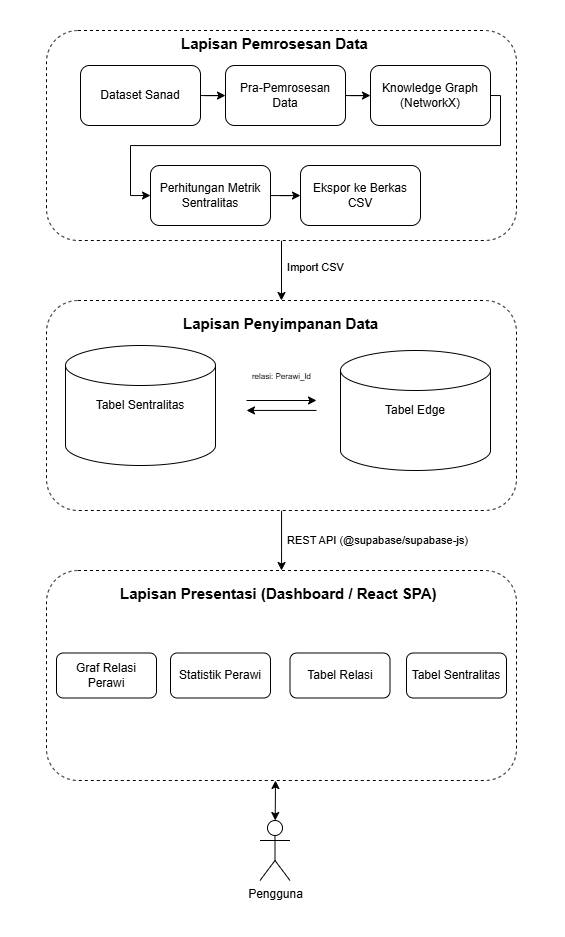
\includegraphics[width=0.78\columnwidth]{contents/chapter-3/Arsitektur-sistem.png}
\caption{Three-tier system architecture separating offline analysis, centralized
storage, and the interactive presentation layer.}
\label{fig:arsitektur}
\end{figure}

The force-directed layout combines three forces per animation frame: a
Coulomb-like \emph{repulsion} $F_r = k_r/d^2$ ($k_r = 2000$) applied between node
pairs closer than 320~px, a Hooke-like \emph{spring} force
$F_s = (d - L_0)k_s$ ($L_0 = 200$~px, $k_s = 0.003$) along edges, and a
\emph{radial constraint} $F_c = (r - r_{target})k_c$ ($k_c = 0.014$) that pulls
each node toward a concentric ring keyed to its centrality rank, so the most
central narrators settle near the graph center. Velocities are damped by a factor
of 0.78 per frame. Centrality is further encoded through node size (28, 20, 14,
10, and 7~px by rank group) and color, and edges are drawn as arrows pointing from
student to teacher.

\subsection{Testing and Evaluation}

Four complementary evaluations were performed. \emph{Black-box testing} covered 14
scenarios spanning navigation, data loading, graph rendering, node selection,
metric filtering, search, zoom, drag and pan, auto-fit reset, the statistics page,
both tables, pagination, and sorting.

\emph{Non-functional testing} follows the \textit{Performance Efficiency}
characteristic of ISO/IEC~25010 as applied to web information systems by Rajata
\textit{et al.}\ \cite{Rajata2026SPP}, covering \textit{Time Behaviour},
\textit{Resource Utilization}, and \textit{Capacity}. Frame rate was sampled once
per second through a Playwright-injected frame counter during zoom, pan, and node
drag, and judged against the common thresholds of 60~FPS for smooth animation and
30~FPS for perceptible jank \cite{Zhao2025}. Browser memory was measured as the
active JavaScript heap via the Chrome DevTools Protocol
(\texttt{Performance.getMetrics}) with forced garbage collection before each
reading, at node counts $N$ increasing toward full network scale. API load testing
used k6 against the Supabase REST endpoints with a ramping virtual-user (VU)
profile, with success criteria of p(95) latency below 1{,}000~ms and a request
failure rate below 1\%.

\emph{Usability evaluation} used an online questionnaire adapting seven of the ten
standard System Usability Scale (SUS) statements \cite{Brooke1996}, omitting the
three items on cumbersomeness, user confidence, and prior learning. Because the
item count differs, the standard multiplier of 2.5 does not apply: per-item
contributions were computed as usual (positive items as response minus~1, negative
items as 5~minus response), and the resulting 0--28 total was rescaled to 0--100
by a factor of $100/28$. The result is therefore an \emph{adapted} SUS score, not
a standard one. Eighteen respondents completed the questionnaire, which also
collected demographics and three open-ended questions.

% =============================================================
\section{Results and Discussion}
% =============================================================

\begin{figure*}[!t]
\centering
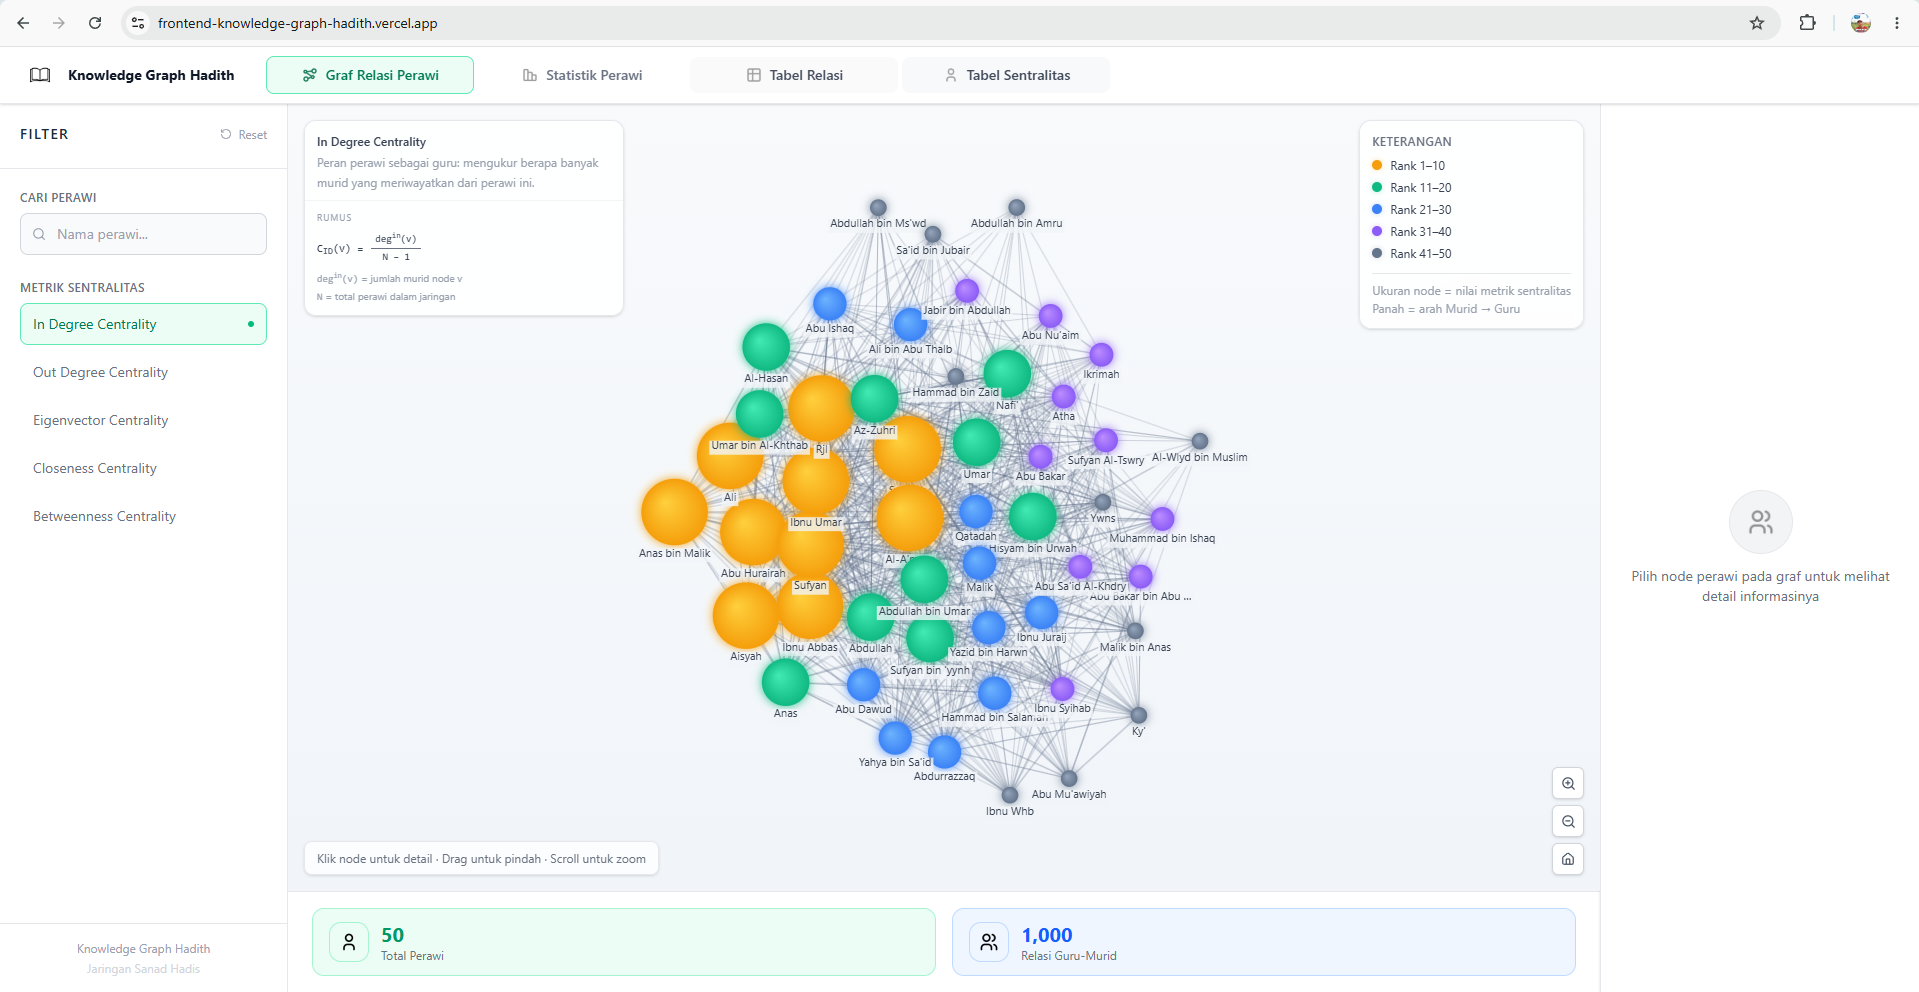
\includegraphics[width=0.92\textwidth]{contents/chapter-4/Tampilan1.png}
\caption{Narrator Relation Graph page of the dashboard. Node size and color encode
centrality rank (In-degree selected); arrows point from student to teacher. The
left panel filters by metric and search; the right panel shows per-narrator
detail when a node is selected.}
\label{fig:dashboard}
\end{figure*}

\subsection{Graph Construction and Structure}

Normalization yielded 177{,}289 unique narrator names; of these, 177{,}047
participate in at least one narration relation and form the graph nodes, the
remaining 242 being isolated names (single-narrator chains or names dropped
during self-loop and empty-name cleaning). The resulting directed graph contains
177{,}047 nodes and 776{,}798 edges. The strongest relation is Ibnu
Umar~$\leftarrow$~Nafi' with a weight of 11{,}346, indicating that Nafi'
narrated from Ibnu Umar that many times in the corpus; such high-weight pairs
form a dominant transmission backbone that recurs across many chains.

Table~\ref{tab:struktur} reports the structural profile. The density of
$2.478 \times 10^{-5}$ marks the graph as sparse: each narrator connects directly
to 8.775 others on average out of 177{,}046 possible partners, characteristic of
large real-world social networks. A single weakly connected component holds
99.91\% of all nodes, so the \textit{sanad} network is one interconnected
structure rather than isolated islands of transmission. Strongly connected
components are far more numerous (47{,}300), consistent with the one-way nature of
narration: mutual reachability requires a directed teacher--student path in the
same direction, which is far rarer. The approximate diameter of 28 on the largest
component indicates that the longest path between any two narrators remains short
relative to a network of this size, consistent with small-world behavior.

\begin{table}[!t]
\caption{Structural Characteristics of the Sanad Graph}
\label{tab:struktur}
\centering
\renewcommand{\arraystretch}{1.3}
\begin{tabular}{lr}
\toprule
Parameter & Value \\
\midrule
Density                              & $2.478 \times 10^{-5}$ \\
Mean node degree                     & 8.775 \\
Weakly connected components          & 51 \\
Largest weakly connected component   & 176{,}891 (99.91\%) \\
Strongly connected components        & 47{,}300 \\
Largest strongly connected component & 129{,}721 \\
Approximate diameter (largest WCC)   & 28 \\
\bottomrule
\end{tabular}
\end{table}

\subsection{Computational Performance of Graph Construction and Analysis}

Table~\ref{tab:bench} reports the cost of each pipeline stage on the full graph.
Data loading, graph construction, and the four degree- and eigenvector-based
metrics together take roughly 13~s at negligible memory cost. Closeness and
betweenness are dramatically more expensive---about 9.4 and 3.8~minutes
respectively---\emph{even under sampling} at $k=100$ rather than exact computation
over all 177{,}047 nodes. Extrapolating from the sampled timings, exact
betweenness on the full graph would require more than 50~hours, which quantitatively
confirms the methodological decision to restrict both path-based metrics to the
14{,}695-node representative subgraph. Peak process memory reached only 701.4~MB
on a 6.29~GB machine, showing that a 177{,}047-node KG can be built and analyzed
on modest hardware; execution time, not memory, is the binding constraint.

\begin{table}[!t]
\caption{Computational Cost of KG Construction and Analysis}
\label{tab:bench}
\centering
\renewcommand{\arraystretch}{1.25}
\begin{tabular}{lrr}
\toprule
Stage & Time & $\Delta$ RSS \\
\midrule
CSV loading                          & 2.07 s   & $+$172.6 MB \\
Graph construction                   & 4.09 s   & $+$300.9 MB \\
Self-loop removal                    & 0.06 s   & $\approx$0 MB \\
Weighted degree                      & 0.86 s   & $+$1.8 MB \\
Degree centrality                    & 0.19 s   & $+$1.4 MB \\
In-degree centrality                 & 0.16 s   & $\approx$0 MB \\
Out-degree centrality                & 0.15 s   & $\approx$0 MB \\
Eigenvector centrality               & 5.10 s   & $+$7.3 MB \\
Closeness centrality (sampled, $k$=100)   & 562.83 s & --- \\
Betweenness centrality (sampled, $k$=100) & 228.57 s & --- \\
\midrule
\multicolumn{2}{l}{\textbf{Peak process memory (peak RSS)}} & \textbf{701.4 MB} \\
\bottomrule
\end{tabular}
\end{table}

\subsection{Residual Ambiguity of Kinship Resolution}

Kinship resolution fired 102{,}100 times across the 487{,}451 chains, dominated by
\textit{Abihi} (``his father,'' 93{,}066 events, 91.1\%), followed by
\textit{Jaddihi} (7{,}287, 7.1\%), \textit{Ummihi} (1{,}004, 1.0\%),
\textit{Abiha} (425, 0.4\%), \textit{Jaddatihi} (234, 0.2\%), and \textit{Abaihi}
(84, 0.1\%). These events produced 14{,}231 string-unique nodes, an average of
7.17 events per node. That average alone does not indicate identity collision,
since a canonical \textit{isnad} quoted identically across many books produces the
same repetition. After classification by anchor specificity, only 623 of 14{,}231
nodes (4.4\%) carry bare anchors---yet this small group accounts for 10{,}059 of
102{,}100 events (9.85\%), a disproportionate share. The highest-frequency
collision candidates include \textit{Abu Salim}, \textit{Abu Mu'tamir},
\textit{Abu Rajul}, \textit{Abu Sufyan}, \textit{Umm Al-Hasan}, \textit{Abu
Ibrahim}, \textit{Abu Jaddi}, and \textit{Abu Ahmad}.

The degree comparison in Table~\ref{tab:kinship} makes the effect visible on the
graph itself. A naive comparison of all resolved nodes against direct nodes,
without distinguishing anchor specificity, shows no significant difference (mean
8.33 vs.\ 8.81; median 2 vs.\ 2; Mann-Whitney~U $p = 0.275$), which would have
suggested that kinship resolution does not inflate degree at all. Splitting by
anchor specificity reverses that reading: bare-anchor nodes average a degree of
66.71, far above both other groups, with very strong statistical significance
($p \approx 4\times10^{-45}$ against direct nodes and $p \approx 7\times10^{-47}$
against qualified-anchor nodes), while qualified-anchor resolved nodes are in fact
slightly \emph{lower} in degree than direct nodes ($p = 0.99$).

\begin{table}[!t]
\caption{Graph Degree by Node Group}
\label{tab:kinship}
\centering
\renewcommand{\arraystretch}{1.3}
\begin{tabular}{lrrr}
\toprule
Group & Nodes & Mean deg. & Median deg. \\
\midrule
Direct                        & 162{,}874 & 8.81  & 2 \\
Resolved (qualified anchor)   & 13{,}552  & 5.66  & 2 \\
Resolved (bare anchor)        & 621       & 66.71 & 4 \\
\bottomrule
\end{tabular}
\end{table}

Manual inspection agrees. \textit{Abu Salim} (1{,}492 events, degree 625) is
dominated by ``\textit{Salim `an abihi}'' chains through Az-Zuhri, most likely
Salim bin Abdullah bin Umar, consistently leading to Umar bin Khattab---but a
minority tail leads to Hafshah, Zaid bin Tsabit, and a different \textit{Salim},
indicating partial contamination. \textit{Abu Mu'tamir} (234 events, degree 126)
shows a far more heterogeneous successor distribution across roughly 80 books, a
stronger collision signal. By contrast \textit{Abu Hisyam bin Urwah} (6{,}562
events), a qualified anchor, consistently denotes one individual despite being
among the most frequent, confirming that frequency alone is not a reliable
indicator.

Taken together, the risk is measurable and concentrated rather than pervasive:
9.85\% of resolution events carry high merge risk, while the remaining 90.15\%
behave statistically like direct-name nodes. The 4.4\% bare-anchor share of
resolved nodes can therefore be reported as an upper bound on identity-collision
risk, in place of an unevidenced claim that all resolved names are ambiguous.

\subsection{Centrality Analysis}

Table~\ref{tab:topnarrators} lists the top narrators for each metric. Abu
Hurairah ranks first in four of five metrics---in-degree, eigenvector, closeness,
and betweenness---identifying him as the most central and most influential
narrator in the network. Sufyan ranks first in out-degree, reflecting a distinct
role as an exceptionally active recipient who narrated from many teachers; the
divergence between the in-degree and out-degree rankings confirms that dominant
sources of narration are not necessarily the most active receivers.

\begin{table}[!t]
\caption{Top Narrators by Centrality Metric}
\label{tab:topnarrators}
\centering
\renewcommand{\arraystretch}{1.3}
\begin{tabular}{cllc}
\toprule
Rank & Metric & Narrator & Score \\
\midrule
1 & In-degree    & Abu Hurairah          & 0.0199 \\
2 & In-degree    & Ibnu Abbas            & 0.0150 \\
3 & In-degree    & Aisyah                & 0.0132 \\
\midrule
1 & Out-degree   & Sufyan                & 0.0135 \\
2 & Out-degree   & Abu Abdullah Al-Hafizh & 0.0127 \\
3 & Out-degree   & Syu'bah               & 0.0124 \\
\midrule
1 & Eigenvector  & Abu Hurairah          & 0.5195 \\
2 & Eigenvector  & Aisyah                & 0.4836 \\
3 & Eigenvector  & Ibnu Umar             & 0.3821 \\
\midrule
1 & Closeness    & Abu Hurairah          & 1.0000 \\
2 & Closeness    & Aisyah                & 0.9965 \\
3 & Closeness    & Ibnu Abbas            & 0.9864 \\
\midrule
1 & Betweenness  & Abu Hurairah          & 0.0500 \\
2 & Betweenness  & Syu'bah               & 0.0445 \\
3 & Betweenness  & Sufyan                & 0.0384 \\
\bottomrule
\end{tabular}
\end{table}

The eigenvector scores drop sharply after the top four narrators (from 0.2659
for Ibnu Abbas to 0.1723 for Anas), indicating that influence is concentrated in
a small, tightly interconnected core. Closeness scores among the top ten are very
high and closely spaced (0.9630--1.0000) because, within the strongest-weight
subgraph, central narrators reach others through very short paths. In
betweenness, the recurrence of Abu Hurairah, Syu'bah, and Sufyan among the top
ranks signals a dual role as both influential and connective nodes.

\subsection{Historical Interpretation of the Dominance Pattern}

The structural dominance recovered by the metrics aligns with the classical
biographical record. Nawawi \cite{Nawawi2024} records that Abu Hurairah narrated
5{,}374 hadith, the highest of any companion, far ahead of Abdullah bin Umar
(2{,}630) and Aisyah (2{,}210). Two historical factors explain that volume---his
full-time attendance on the Prophet as one of the \textit{Ashabu al-Suffah},
unencumbered by worldly occupation, and a memorization capacity that classical
reports associate with a specific supplication of the Prophet \cite{Nawawi2024}.
Structurally, this manifests as the node with the most receiving students and the
broadest connectivity to other influential narrators.

Sufyan's dominance, by contrast, is confined to out-degree---the metric counting
distinct teachers as sources---which matches his historical reputation as an
outstanding \emph{recipient} rather than a center of instruction. Among the
classical assessments compiled by Rokhibi \textit{et al.}\ \cite{Rokhibi2025},
Yahya bin Ma'in held that no one knew the hadith of Al-A'mash better than Sufyan
al-Thawri, and Ibnu Abi Khaitsamah relayed his father's judgment that Sufyan
al-Thawri was Al-A'mash's most \textit{ahfaz} student. His standing was thus built
on receiving narration with high precision rather than on being a reference for
many students, exactly the asymmetry the directed graph exposes. This
identification takes ``Sufyan'' to be Sufyan al-Thawri as the most prominent
bearer of that name in classical transmission, since the dataset does not carry
full \textit{nasab} to confirm a single identity.

Both patterns reinforce a principle of hadith scholarship: a narrator's role
cannot be reduced to one number, but is understood through position within the
chain, as traditionally studied through \textit{rijal} and \textit{tabaqat}
literature. Distinguishing relation direction through in-degree and out-degree
reproduces quantitatively, across 177{,}047 narrators, the role distinction that
classical scholars mapped qualitatively.

\subsection{Dashboard Implementation}

The analytical results were stored in Supabase and served through the React
dashboard. Fig.~\ref{fig:dashboard} shows the Narrator Relation Graph page, the
core of the system, rendering narrators as nodes and teacher--student relations as
directed edges on an HTML5 Canvas. A left filter panel provides search and the
five centrality metrics; selecting a metric drives node size and color so that
the most central narrators appear largest and centered, while an overlay card
updates to show the selected metric's formula and the narrator role it measures,
addressing the semantic-accessibility requirement. For readability the view
displays a representative subset of the top 50 narrators with 1{,}000 relations.
Selecting a node opens a right-hand detail panel with the narrator's connected
teacher and student counts, all five centrality values, and the linked narrators,
while highlighting the node's direct relations. The graph supports zoom, pan,
drag, node selection, and auto-fit reset.

The remaining three pages complement this view. The \emph{Narrator Statistics}
page summarizes the network with total-narrator (177{,}047) and total-relation
(776{,}798) indicator cards and five bar charts of the top ten narrators per
metric. The \emph{Relation Table} page lists all 776{,}798 weighted
teacher--student relations across 777 pages with pagination, sorting, and search;
by default it is sorted by weight, placing Ibnu Umar--Nafi' (11{,}346) at the top.
The \emph{Centrality Table} page lists all 177{,}047 narrators with their five
centrality scores across 178 pages, also paginated, sortable, and searchable. The
dashboard was deployed online and is publicly accessible without installation.

\subsection{Functional Testing and Output Validity}

All 14 black-box scenarios produced the expected output, a 100\% success rate, so
the dashboard required no corrective iteration between design and build. The
scenarios fall into three groups: navigation and data loading (1--2), the
Narrator Relation Graph page including selection, metric filtering, search, zoom,
drag, and reset (3--9), and the statistics and table pages with pagination and
sorting (10--14).

Functional testing confirms that a feature displays data, not that the displayed
data is sound, so output validity was examined on three additional levels. On
\emph{input validity}, name normalization prevents one narrator from splitting
across several nodes, while the converse risk---several narrators merging into one
node---was quantified at 9.85\% of resolution events rather than assumed absent.
On \emph{presentation consistency}, the dashboard never recomputes centrality
client-side but reads precomputed values from Supabase, and the data-loading
scenario verified that displayed values match database contents. On \emph{external
validity}, the narrators the system identifies as most central agree with
independent manual scholarship, as detailed in Section~\ref{sec:compare}.

\subsection{Non-Functional Performance}

Frame rate stayed comfortably above the jank threshold in all three interactions
(Table~\ref{tab:fps}). Zoom averaged 57.0~FPS with a 51~FPS minimum, slightly
below pan (61.0) and node drag (60.7), consistent with zoom recomputing view
transform and scale on every scroll-wheel event in addition to carrying the same
per-frame physics and render load as the others. The difference is measurable but
too small to be perceived as stutter.

\begin{table}[!t]
\caption{Frame Rate During Graph Interaction}
\label{tab:fps}
\centering
\renewcommand{\arraystretch}{1.3}
\begin{tabular}{lcc}
\toprule
Scenario & Mean FPS & Min FPS \\
\midrule
Zoom in/out (scroll wheel) & 57.0 & 51 \\
Pan canvas                 & 61.0 & 60 \\
Drag one node              & 60.7 & 60 \\
\bottomrule
\end{tabular}
\end{table}

Browser memory did not scale proportionally with node count over the range that
could be tested, staying between 8.8 and 11.1~MB from $N=50$ to $N=500$
(Table~\ref{tab:memori}). At $N=1{,}000$---still under 1\% of the 177{,}047
narrators in the network---the request never completed within the observation
window. Memory usage at full network scale therefore cannot be measured
empirically on the current architecture, because data fetching fails long before
that scale is reached. This makes the decision to render a representative
50-node subset a matter of architectural capacity as much as visual readability.

\begin{table}[!t]
\caption{Browser Heap Usage vs.\ Node Count}
\label{tab:memori}
\centering
\renewcommand{\arraystretch}{1.3}
\begin{tabular}{ccc}
\toprule
$N$ (requested) & Nodes received & Heap usage \\
\midrule
50      & 50      & 8.8 MB \\
100     & 100     & 11.1 MB \\
250     & 250     & 10.1 MB \\
500     & 500     & 10.3 MB \\
1{,}000 & Total failure & --- \\
\bottomrule
\end{tabular}
\end{table}

Load testing over a 95~s ramp of $0\rightarrow10\rightarrow50\rightarrow100
\rightarrow0$ VUs failed the p(95) latency threshold---4.68~s actual against a
1{,}000~ms target, with a 1.31~s mean and a 12.72~s maximum---while passing the
failure-rate threshold with 0\% failures (2{,}300 of 2{,}300 checks) at an average
throughput of 23.9 requests/s. The fixed-stage breakdown in
Table~\ref{tab:load} locates the limit: the system meets the 1~s target only at 10
concurrent users (p95 595~ms); at 50 VUs p95 has already reached 2.76~s. At 100
VUs throughput actually falls from 29.1 to 27.7 requests/s while p95 climbs to
7.63~s, the signature of saturation---requests queue rather than being rejected,
which is why the failure rate remains 0\% instead of returning 429 codes. The
practical breaking point therefore lies between 10 and 50 concurrent users on the
Supabase tier used. These three tests were run with shortened repetition counts
for initial verification, so the figures are valid preliminary measurements that
warrant larger-sample repetition before being treated as final.

\begin{table}[!t]
\caption{Load Testing per Fixed VU Stage (20 s each)}
\label{tab:load}
\centering
\renewcommand{\arraystretch}{1.3}
\begin{tabular}{ccccc}
\toprule
VU & Throughput & P95 latency & Max latency & Failure rate \\
\midrule
10  & 12.6 req/s & 595 ms  & 1.11 s  & 0\% \\
50  & 29.1 req/s & 2.76 s  & 7.43 s  & 0\% \\
100 & 27.7 req/s & 7.63 s  & 15.29 s & 0\% \\
\bottomrule
\end{tabular}
\end{table}

\subsection{Usability Evaluation}

All 18 respondents were aged 20--25, and only one (5.6\%) had an academic or
professional background in hadith studies, so the results reflect general-user
perception rather than the primary target audience and should be read as a
preliminary indication. Ten respondents (55.6\%) rarely used comparable graph
visualization applications and four (22.2\%) never had.

Item means were highest for feature integration (4.33) and ease of use (4.22),
and lowest for the negatively worded inconsistency item (2.06)---a positive
result, since low agreement there means respondents did not perceive
inconsistency. The adapted SUS statistics appear in Table~\ref{tab:sus}: a mean of
71.23 on a 0--100 scale, above the scale midpoint, with substantial spread
(SD~15.85, range 35.71--92.86). Given the seven-item instrument and the respondent
profile, this score is best read as an early positive signal rather than a
standard, target-audience-representative measure.

\begin{table}[!t]
\caption{Adapted SUS Scores (7 Items, $n=18$)}
\label{tab:sus}
\centering
\renewcommand{\arraystretch}{1.3}
\begin{tabular}{lc}
\toprule
Statistic & Value \\
\midrule
Respondents ($n$) & 18 \\
Mean              & 71.23 \\
Median            & 73.22 \\
Standard deviation & 15.85 \\
Minimum           & 35.71 \\
Maximum           & 92.86 \\
\bottomrule
\end{tabular}
\end{table}

Open-ended responses named the interface design, the ease of tracing
teacher--student relations through the graph, and the search and click-through
features as what respondents liked most. The most frequent obstacles were the
absence of onboarding guidance and unfamiliarity with what the centrality metrics
mean, followed by label crowding when the graph is dense---and the suggestions
matched: add metric explanations or tooltips, and reduce label overlap.

\subsection{Comparison with Prior Work}
\label{sec:compare}

Table~\ref{tab:compare} positions this work against prior \textit{sanad} network
studies. Earlier work successfully models and analyzes narrator networks at
scale, but the outputs are typically static and tied to desktop software such as
Gephi and Cytoscape, restricting access to expert users
\cite{FAROOQI2024110439,Shuaib2022}. The principal advantage of this work is the
presentation of the analysis as an interactive, publicly accessible web dashboard
that integrates a large-scale narrator KG with all five centrality metrics and
exploration features in a single interface.

\begin{table}[!t]
\caption{Comparison with Prior Sanad Network Studies}
\label{tab:compare}
\centering
\renewcommand{\arraystretch}{1.3}
\begin{tabular}{p{1.95cm}ccccc}
\toprule
Study & KG & SNA & Web & Public & Perf. \\
\midrule
Farooqi \textit{et al.}~\cite{FAROOQI2024110439}   & Yes & Partial & No  & No  & No \\
Shuaib \textit{et al.}~\cite{Shuaib2022}           & No  & No      & No  & No  & No \\
Mahmoud \textit{et al.}~\cite{Mahmoud2024}         & Yes & No      & No  & No  & No \\
Ahmad \textit{et al.}~\cite{ahmad2025hadith}       & Yes & Yes     & No  & No  & No \\
KASHAF~\cite{shafie2021kashaf}                     & Yes & No      & Yes & Partial & No \\
\textbf{This work} & \textbf{Yes} & \textbf{Yes} & \textbf{Yes} & \textbf{Yes} & \textbf{Yes} \\
\bottomrule
\end{tabular}
\end{table}

A direct numerical comparison of computational efficiency against Neo4j
\cite{FAROOQI2024110439} or NarratorsKG \cite{Mahmoud2024} is not possible,
because both publications focus on dataset construction and disambiguation
accuracy---Farooqi \textit{et al.}\ report a graph of 2{,}092 nodes and 77{,}797
edges, and Mahmoud \textit{et al.}\ report 95.2\% accuracy with a 23.2\%
\textit{sanad} error rate---without measuring processing time, query latency, or
any other efficiency metric for the graph systems they build. This work supplies
those missing figures at a scale of 177{,}047 narrators: about 13~s to build the
full graph and compute the degree- and eigenvector-based metrics, and a 595~ms P95
API latency at 10 concurrent users.

The centrality results also agree with independent manual scholarship. Mufid and
Sattar \cite{mufid2023track}, applying Motzki's \textit{isnad-cum-matn} method to
a single hadith, found that Abu Hurairah built a far wider \textit{isnad} bundle
than Abu Sa'id al-Khudri. That small-scale qualitative finding is consistent with
the large-scale quantitative result here, which places Abu Hurairah first in four
of five metrics across 177{,}047 narrators. A similar convergence holds for Ibnu
Syihab Az-Zuhri, described by Shuaib \textit{et al.}\ \cite{Shuaib2022} as the
first systematic collector and disseminator of hadith: in this network his
relation with Ma'mar carries the seventh-highest weight overall (4{,}381),
so his central position is detected structurally as well.

Finally, this work carries out the analysis that Farooqi \textit{et al.}\
\cite{FAROOQI2024110439} explicitly identified as applicable to their dataset but
left undone, executing it directly at full scale on 177{,}047 narrators.

\subsection{Limitations}

Closeness and betweenness centrality were computed on the strongest-weight
subgraph rather than the full graph due to computational cost; the dataset is
static and not automatically updated; and the analysis addresses network structure
without assessing \textit{sanad} authenticity from the perspective of hadith
science. On the implementation side, the current data-fetching architecture cannot
load a graph approaching full scale, so the display remains limited to a
representative subset. The usability evaluation is constrained on two counts: only
1 of 18 respondents came from a hadith-studies background, and the questionnaire
adapts seven of the ten standard SUS items, so its score cannot be compared
against standard 10-item interpretation thresholds. Name validity was likewise not
verified exhaustively, so some entries remain generic terms rather than genuine
narrator names.

% =============================================================
\section{Conclusion}
% =============================================================

This paper analyzed the Islamic scholarly network of the hadith \textit{sanad}
using a Knowledge Graph with Social Network Analysis and presented the results
through an interactive web dashboard. From the Sanadset~650K corpus, 487{,}451
cleaned \textit{sanad} chains were modeled as a weighted directed graph of
177{,}047 narrator nodes and 776{,}798 narration edges; the residual risk of
identity merging from kinship resolution was quantified at 9.85\% of resolution
events rather than left as an untested assumption.

The weighted directed representation proved effective at exposing key narrator
roles that conventional text search cannot reach. Text search yields one
occurrence count, whereas the five centrality metrics decompose that single number
into distinct structural roles: Abu Hurairah ranks first in four of five metrics,
while Sufyan and Syu'bah stand out specifically in out-degree and betweenness---a
role distinction impossible to recover from frequency alone, and one that agrees
with independent manual scholarship.

The results are served through a React and Supabase dashboard that is publicly
accessible without installation. Validation spanned three complementary aspects:
14 black-box scenarios at a 100\% success rate, non-functional testing showing
adequate graph rendering performance (57--61~FPS) and API resilience with a
practical breaking point between 10 and 50 concurrent users, and an adapted SUS
evaluation with 18 respondents averaging 71.23.

Future work should compute closeness and betweenness on the full graph using
approximation algorithms or parallel computation; incorporate periodic data
updates and additional \textit{sanad} sources; disambiguate bare-anchor nodes
against biographical (\textit{rijal}/\textit{tabaqat}) sources and complete the
prepared 150-row gold-standard review to obtain citable precision and recall; and
repeat the usability evaluation with hadith students and researchers using the
full 10-item SUS instrument plus task-based testing. The full-scale graph built
here also opens the way to Graph Neural Network approaches for link prediction,
estimating missing narrators in broken (\textit{mursal}/\textit{munqati'}) chains,
extending the text-based continuity verification of Hendawi \textit{et al.}\
\cite{10974901} to a structural setting.

\section*{Acknowledgment}

The authors thank the Department of Electrical and Information Engineering,
Universitas Gadjah Mada, for supporting this research, and acknowledge Mghari
\textit{et al.}\ for publicly releasing the Sanadset~650K dataset.

\bibliographystyle{IEEEtran}
\bibliography{references}

\end{document}
